\documentclass[11pt]{article} 

../macros/macros.tex

% \renewcommand{\capac}[1]{\ensuremath{\operatorname{\sf cap}(#1)}}
% \newcommand{\rescap}[1]{\ensuremath{\operatorname{\sf cap}_f(#1)}}
% \newcommand{\into}[1]{\ensuremath{\operatorname{\sf in}(#1)}}
% \newcommand{\out}[1]{\ensuremath{\operatorname{\sf out}(#1)}}

% \newenvironment{LP}[1]{
%   \begin{array}[t]{@{}l@{}}
%     \displaystyle #1 \\
%     \begin{aligned}\\[-10pt]}{\end{aligned}\end{array}}


% \newenvironment{myframed}
% {\smallskip\par\noindent\begin{minipage}{\textwidth}\begin{framed}\vspace*{-5pt}}{\vspace*{-5pt}\end{framed}\end{minipage}\smallskip}

\begin{document}

\doTitle{9}{The complexity classes P and NP}{P and NP}

\newpage

\section{Intractable computational problems}\label{np: sec: intro}\doHeader{Intractable problems}
% \paragraph{Computational intractability.}
Many important computational problems are \emph{intractable} ---
not solvable by any reasonably fast algorithm.
Since 1950 or so, computer scientists have developed
a fairly deep understanding of intractable problems.

In designing algorithms, it is useful to be able tell when a problem is intractable,
or likely to be intractable.
If your problem is intractable,
there is no algorithm that is guaranteed
to compute a correct solution to every input in reasonable time.
In this case, you need some other approach.
For example, perhaps you only care about solving a few particular instances
of the problem.  Then you might focus on solving just those instances.
Or, you might look for fast algorithms that are guaranteed to
return provably good \emph{approximate} solutions.
Or, you might revisit your application and try to
find a different way to formally model what you need to do.

We focus here on a particular kind of intractability:
whether or not the problem has any algorithm
whose worst-case running time is bounded by \emph{any polynomial} ---
that is, for some constant $c>0$, on any input $x$,
the algorithm takes time $O(|x|^c)$.
The class of problems that have such algorithms is called \emph{Polynomial Time},
and is often denoted P (or $\mathbb{P}$).
Note that this is a class of \emph{problems}, not algorithms.
P is one of many \emph{complexity classes} studied by computer scientists.

We also focus on another particular class of algorithmically important problems,
so-called ``NP-complete'' problems.
We have \emph{strong evidence} that these problems
are not in P
(have no polynomial-time algorithms)
so, are very likely to be intractable in that sense.

\section{Reductions revisited}\label{np: sec: reductions}\doHeader{Reductions}
\LN{flow} formally defined polynomial-time reductions,
and gave reductions from \prob{Bipartite Matching} to \prob{Max Flow},
from \prob{Disjoint Paths} to \prob{Max Flow},
from \prob{Max Flow} to \prob{Linear Programming},
and from \prob{Shortest $s$-$t$ Path} to \prob{Linear Programming}.
These enable us to, for example, use any algorithm for \prob{Linear Programming}
to solve \prob{Shortest $s$-$t$ Path}, \prob{Max Flow}, and
\prob{Bipartite Matching}.

Recall that when considering reductions we focus on \emph{decision problems} ---
computational problems with `yes'/`no' answers.
For any decision problem $A$, we define the \emph{language}, $L(A)$ associated with $A$
to be the set of inputs for which the answer is ``yes''.  For example, the language
for the decision problem for \prob{Shortest $s$-$t$ Path}
is the set
\[L = \{ (G, s, t, W) \giv \text{there is an $s$-$t$ path in $G$ of weight at most $W$}\}.\]
To be formally precise,
we have in mind here that each input is encoded in a standard way
as a binary string. So, each language is, technically, a set of binary strings.
But we can safely forget about this most of the time.
It is important mainly in that it gives us a robust and general notion of input size
--- the size of an input is the number of bits in the encoding of the input.

If an algorithm for a decision problem $A$ says `yes' for a given input $x$,
we say the algorithm \emph{accepts} $x$.  
So, if the algorithm is correct, then, for all inputs $x$
the algorithm accepts $x$ if and only if $x\in L(A)$.

Recall from \LN{flow} that a reduction from a decision problem $A$ (such as \prob{Bipartite Matching})
to another decision problem $B$ (such as \prob{Max Flow})
is, formally, a function $r$
such that, given any input $x$ for problem $A$,
the function produces an equivalent instance $r(x)$ of problem $B$.
\emph{Equivalent} means that $x$ is in $L(A)$
if and only if $r(x)$ is in $L(B)$.
The reduction is a \emph{polynomial-time} reduction if the function $r$ can be computed in polynomial time.
That is, there is an algorithm that, given input $x$, outputs $r(x)$ in time polynomial in $|x|$.
Recall that the notation \[
  A \le_P B
\] means that there is a polynomial-time reduction from $A$ to $B$.
Informally, it means that $A$ is ``no harder'' than $B$.
(To be more precise, $A$ is at most ``polynomially harder'' than $B$.)
Recall the following lemmas from \LN{flow}:

\begin{lemma}\label{np: reduction}
  Let $A$ and $B$ be decision problems
  such that $A$ reduces in polynomial time to $B$.
  If $B$ has a polynomial-time algorithm,
  then $A$ has a polynomial-time algorithm.
  That is, if $A \le_P B$ and $B\in P$, then $A\in P$.
\end{lemma}

\begin{lemma}\label{np: transitive}
  Let $A$, $B$, and $C$ be decision problems.
  If $A$ reduces in polynomial time to $B$,
  and $B$ reduces in polynomial time to $C$,
  then $A$ reduces in polynomial time to $C$.

  That is, if $A\le_P B$ and $B\le_P C$, then $A\le_P C$.
\end{lemma}

\section{Reductions between some problems that are new to us}\label{np: sec: reductions 2}\doHeader{More reductions}

\subsection{Three similar problems: Clique, Independent Set, and Vertex Cover}
Given an undirected graph $G=(V,E)$,
a \emph{clique} is a subset $K\subseteq V$ of the vertices such that every
% [review 2026-09-27] fix: the clique was named K but the condition referred to C; changed C to K
pair of vertices in $K$ has an edge in $E$.
An \emph{independent set} is a subset $I\subseteq V$ of the vertices such that
no pair of vertices in $I$ has an edge in $E$.
A \emph{vertex cover} is a subset $C\subseteq V$ of the vertices such that
every edge in $E$ has an endpoint in $C$.
Here are the three corresponding decision problems.

For each, the input is $G=(V,E)$ and an integer $k$.
\begin{description}
\item[\prob{Clique} ---] does $G$ have a clique of size $k$ or more?
\item[\prob{Independent Set} ---] does $G$ have an independent set of size $k$ or more? 
\item[\prob{Vertex Cover} ---] does $G$ have a vertex cover of size $k$ or less?
\end{description}

Each of these three problems reduces in polynomial time to each of the others.

\paragraph{Reducing Clique to Independent Set.} 
Here is a reduction $f_1$ of \prob{Clique} to \prob{Independent Set}.
Given an instance $(G=(V,E),k)$ of \prob{Clique},
define $f_1(G,k)$ to be the instance $(\overline G, k)$ of {\sc Independent Set},
where $\overline G = (V, \overline E)$
has the same vertex set of $G$, and has exactly those edges that $G$ does not have.

To verify correctness, observe that $f_1$ can be computed in time polynomial in the size of its input,
and that, for all instances $(G,k)$ of \prob{Clique},
the answer to $(G,k)$ is ``yes''
($G$ has a clique of size at least $k$)
if and only if
the answer to the instance $f_1(G,k)$ of \prob{Independent Set} is ``yes''
($\overline G$ has an independent set of size at least $k$).
This is because a set $S$ of vertices is a clique in $G$
iff $S$ is an independent set in $\overline G$.

\paragraph{Reducing Independent Set to Clique.}
The function $f_1$ also happens to be a poly-time reduction in the other direction:
from {\sc Independent Set} to \prob{Clique}.

\paragraph{Reducing Independent Set to Vertex Cover.} 
Here is a reduction $f_2$ of \prob{Independent Set} to \prob{Vertex Cover}.
Given an instance $(G=(V,E), k)$ of \prob{Independent Set},
define $f_2(G,k)$ to be the instance $(G, k')$ of \prob{Vertex Cover}, where $k' = |V|-k$.
To verify correctness, observe that $f_2$ can be computed in time polynomial in the size of its input,
and that, for all instances $(G,k)$ of \prob{Independent Set},
the answer to $(G,k)$ is ``yes''
($G$ has an independent set of size $k$)
if and only if
the answer to the instance $f_2(G,k)$ of \prob{Vertex Cover} is ``yes''
($G$ has a vertex cover of size at most $k'=|V|-k$).
This is because a set $S$ of vertices is an independent set in $G$
iff the complement $V\setminus S$ of $S$ is a vertex cover in $G$.

\paragraph{Reducing Vertex Cover to Independent Set.}  
The function $f_2$ also happens to be a poly-time reduction in the other direction:
from {\sc Vertex Cover} to \prob{Independent Set}.

\paragraph{Reducing Clique to Vertex Cover.} 
And, by Lemma~\ref{np: transitive} (reductions compose),
\prob{Clique} reduces to \prob{Vertex Cover} via
the reduction $(G,k) \mapsto f_2(f_1(G,k))$.

\medskip

Thus, we see that all three of these problems are equivalent, in the sense that
if any one of them has a poly-time algorithm, 
then (via the reductions described above)
each of them will have a poly-time algorithm.

It would be reasonable to conclude at this point
that \prob{Clique}, \prob{Independent Set},
and \prob{Vertex Cover} are, in some sense,
just different names for the same problem,
and that is why we can reduce each of these problem to the other.
But the reason is deeper than that.
Next we'll see reductions between problems that, on the surface at least,
are not at all similar.

\subsection{A very different (?) problem: 3-CNF-SAT}
Here are two problems that seem very different from those three:

\begin{description}

\item[\prob{SAT}] ---
  Given a Boolean formula $\phi$,
  is there an assignment of values (true or false) to the variables of $\phi$
  % [review 2026-09-27] fix: an assignment satisfies the formula, not "the assignment"; changed to formula
  that \emph{satisfies} the formula (makes it true).

\item[\prob{3-CNF-SAT} ---] Given a Boolean formula $\phi$ in 3-CNF form (an ``and'' of clauses,
  each of which is an ``or'' of at most three literals, each of which is a variable or its negation),
  is the formula \emph{satisfiable} (that is, can one assign values to the variables to make the 
  formula true).  
  
  For example, 
  $\phi= (x \vee \overline y \vee z) \wedge (y \vee  z) \wedge (\overline y \vee \overline z)$
  is satisfiable: take $x=T$, $y=T$, $z=F$.
\end{description}

We remark that \prob{SAT} is a very ``expressive'' problem --- 
computers are built from logic gates,
so it is not too surprising that Boolean formulae can model computation.
See Lemma 34.6 of the text \CLRS and surrounding discussion for more details.
Also, \prob{SAT} reduces pretty easily to \prob{3-CNF-SAT}.
So \prob{3-CNF-SAT} is just as expressive.

\begin{lemma}
  \prob{3-CNF-SAT}${} \le_p {}$\prob{Independent Set}.
\end{lemma}
\begin{proof}
  Here is the reduction.  Let $\phi$ be any instance of \prob{3-CNF-SAT}.
  Construct the following instance $(G=(V,E), k)$ of \prob{Independent Set}.
  For each variable $x$ in $\phi$,
  introduce a ``variable gadget'' consisting of two new ``literal'' vertices, labeled $x$ and $\overline x$,
  with an edge between them.

  (So far, if there are $h$ variables in $\phi$,
  then there will be $2^h$ independent sets of size $h$.
  Each independent set takes exactly one vertex from each variable gadget,
  and we have in mind that these $2^h$ independent sets
  correspond to the $2^h$ assignments true/false assignments to the variables of $\phi$
  in the natural way.)

  Next, for each clause in $\phi$,
  introduce a ``clause gadget'' consisting of one new vertex for each literal in the clause,
  with edges between each pair of vertices within each clause gadget.
  For example, for the clause $x\vee \overline y \vee z$,
  % [review 2026-09-27] fix: the clause gadget consists of vertices, not variables; changed "variables" to "vertices"
  the clause gadget would consist of three new vertices,
  labeled, respectively, $x$, $\overline y$, and $z$,
  connected by three edges.

  (So far, if there are $h$ variables and $\ell$ clauses in $\phi$,
  each independent set of size $h+\ell$ must contain exactly one vertex from each gadget.)

  Finally, for every vertex $v$ that occurs in each clause gadget,
  introduce an edge between that vertex and the ``opposite'' vertex in the variable gadget.
  For example, if $v$ is labeled with the variable $x$,
  then introduce an edge between $v$ and the vertex labeled $\overline x$ in the variable gadget for $x$.
  Or, if $v$ is labeled with $\overline x$,
  then introduce an edge between $v$ and the vertex labeled $x$ in the variable gadget for $x$.

  This defines the graph $G$.
  Define the threshold $k$ (the desired independent-set size) to be $h+\ell$
  (the number of variables plus clauses, that is, the number of gadgets).
  This defines the reduction:
  $f(\phi) = (G,k)$, where $G$ and $k$ are defined from $\phi$ as described above.  

  Clearly the reduction can be computed in polynomial time.
  That is, given $\phi$, one can construct $G$ and $k$ in time polynomial in $|\phi|$.

  It remains to verify that the reduction $f$ is correct.
  That is, we need to show
  \[(\forall \phi)~~\phi \text{ is satisfiable } \iff (G,k) \text{ has an independent set of size $k$, where } (G,k) = f(\phi).\]
  Above $\phi$ ranges over all instances of 3-CNF-SAT.

  Consider an arbitrary instance $\phi$ of \prob{3-CNF-SAT}.
  
  Let $h$ be the number of variables,
  let $\ell$ be the number of clauses.
  Let $(G,k) = f(\phi)$, so that $k = h+\ell$.
  
  We need to show that
  $\phi$ is satisfiable if and only if $G$ has an independent set of size at least $k$.

  \paragraph{Only if ($\implies$).}  Suppose that $\phi$ is satisfiable.  
  We need to show that in this case $G$ has an independent set $I$ of size at least $k$.
  Fix any assignment $A$ of the variables of $\phi$ that satisfies $\phi$.

  We will describe how to construct $I$ from $A$.
  Make $I$ contain one vertex from each gadget of $G$, as follows.
  For each variable $x$ in $\phi$,
  if $A$ assigns $x$ the value ``true'',
  then make $I$ contain the vertex labeled $x$ from the variable gadget for $x$ in $G$.
  Otherwise
  ($A$ assigns $x$ the value ``false''),
  make $I$ contain the vertex labeled $\overline x$ from the variable gadget.
  For each clause gadget in $\phi$,
  make $I$ contain the vertex from the clause gadget
  that corresponds to some literal in the clause that $A$ makes true
  (there must be at least one such literal, since $A$ satisfies the clause).

  Clearly $I$ has size $k = h+\ell$.
  Also, $I$ is an independent set, because it takes only one vertex from each gadget,
  and (because of the way $G$ is constructed)
  never takes a clause vertex labeled $x$ and a variable vertex labeled $\overline x$,
  or vice versa.

  \paragraph{If ($\impliedby$).} Suppose that $G$ has an independent set of size at least $k=h+\ell$.
  We need to show that in this case $\phi$ has some satisfying assignment $A$.
  Let $I$ be any independent set of size $k$.
  Clearly $I$ has exactly one vertex per gadget in $G$
  (it can't have more than one in any gadget, as each gadget is a clique,
  so it has to have one in each gadget in order to have size $k$).

  Define assignment $A$ from $I$ as follows.
  For each variable $x$, consider the variable gadget for $x$.
  If $I$ takes the vertex labeled $x$, then make $A$ assign $x$ the value ``true''.
  Otherwise ($I$ takes the vertex labeled $\overline x$) make $A$ assign $x$ the value ``false''.
  This defines the assignment.
  To see that it is a satisfying assignment,
  consider any clause of $\phi$.
  $I$ contains some vertex $v$ from the clause gadget,
  where $v$ is labeled with a literal in the clause --- either a variable $x$ or its negation $\overline x$.
  Consider the case when $v$ is labeled with a variable $x$ (the other case is similar).
  There is an edge in $G$ between $v$ 
  and the vertex (call it $v'$) labeled $\overline x$ in $x$'s variable gadget.
  So $v'$ cannot be in the independent set $I$.
  So the vertex labeled $x$ in $x$'s variable gadget has to be in the independent set $I$.
  So the assignment assigns $x$ the value ``true''.
  So the clause is satisfied.
\end{proof}

\section{Review of key concepts}\label{np: sec: review}\doHeader{Review}

The previous reduction is perhaps surprising.
\prob{3-CNF-SAT} reduces to (apparently unrelated) graph problems:
\prob{Independent Set}, \prob{Vertex Cover}, \prob{Clique}.
What's going on?
Let's take stock.
Here's a review of the key concepts so far:

\begin{description}

\item[decision problem] --- A \emph{decision problem} is a computational problem such that, for every input, the answer is either ``yes'' or ``no''.
  In studying computational complexity, we work mostly with decision problems, just to keep things simple.
  Most computational problems can be cast as decision problems.
  
\item[language] --- The \emph{language} associated with a decision problem is the set of inputs for which the answer is ``yes'' (encoded in any standard binary encoding).  We often identify the decision problem with its language.

  An algorithm $A$ for a decision problem is said to \emph{accept} an input $x$ if, on input $x$, $A$ outputs ``yes''.  Otherwise $A$ \emph{rejects} $x$.

\item[polynomial-time algorithm] --- An algorithm runs in \emph{polynomial time} if there is some constant $c>0$ such that the worst-case running time on any input of size $n$ is $O(n^c)$.  Note that this includes, for example algorithms that run in time $O(n\log n)$, because $O(n\log n)$ is $O(n^2)$.

\item[the class P] --- Called \emph{Polynomial Time}, this is the set of decision problems that have polynomial-time algorithms.  This is one of many \emph{complexity classes} studied by computer scientists.  (A complexity class is a collection of computational problems, typically defined as containing all problems that have an algorithm that obeys a some given resource constraint.)

% [review 2026-09-27] fix: the formal restatement said "x in A iff x in B" (wrong: compares x with itself, and A, B are problems, not languages); changed to x in L(A) iff f(x) in L(B), the note's notation from Section 9.2
\item[reduction] --- A \emph{reduction} from a decision problem $A$ to a decision problem $B$ is a function $f$ mapping each input $x$ for $A$ to some input $f(x)$ for $B$, such that the answer for $x$ is ``yes'' if and only if the answer for $f(x)$ is yes.  That is, $(\forall x)~x\in L(A) \iff f(x)\in L(B)$.  When there is a reduction from $A$ to $B$,
  we say \emph{$A$ reduces to $B$}.
  
\item[polynomial-time reduction] --- A reduction $f$ is a \emph{polynomial-time} reduction if there is a polynomial-time algorithm that, given any input $x$, outputs $f(x)$ in time polynomial in $|x|$.  If there is such a reduction,
  we say \emph{$A$ reduces to $B$ in polynomial time}, which we write as $A\le_p B$.
\end{description}

\setcounter{lemma}{0}
\begin{restatement}

\begin{lemma}
  If $A \le_P B$ and $B\in P$, then $A\in P$.
\end{lemma}

\begin{lemma}
  If $A\le_P B$ and $B\le_P C$, then $A\le_P C$.
\end{lemma}

\paragraph{Here are the decision problems we've just considered:}

\begin{description}
  
\item[\prob{Clique} ---]
  % [review 2026-09-27] fix: the review restated Clique as "size k", but Section 9.3.1 defines it as "size k or more"; made the restatement match
  given graph $G$ and integer $k$, does $G$ have a clique of size $k$ or more?

\item[\prob{Independent Set} ---]
  Given $G$ and $k$,
  % [review 2026-09-27] fix: the review restated Independent Set as "size k", but Section 9.3.1 defines it as "size k or more"; made the restatement match
  does $G$ have an independent set of size $k$ or more?

\item[\prob{Vertex Cover} ---]
  Given $G$ and $k$,
  % [review 2026-09-27] fix: the review restated Vertex Cover as "size k", but Section 9.3.1 defines it as "size k or less"; made the restatement match
  does $G$ have a vertex cover of size $k$ or less?

\item[\sc SAT] ---
  Given a Boolean formula $\phi$,
  is there an assignment of values (true or false) to the variables of $\phi$
  % [review 2026-09-27] fix: an assignment satisfies the formula, not "the assignment"; changed to formula
  that \emph{satisfies} the formula (makes it true).

\item[{\sc 3-CNF-SAT} a.k.a.~\sc 3-SAT] ---
  {\sc SAT} restricted to inputs $\phi$ that are in 3-CNF form
  (an ``and'' of clauses, where each clause is an ``or'' of at most three literals,
  where each literal is a variable or the negation of a variable).
  
\end{description}

% [review 2026-09-27] fix: this list was wrapped in a lemma environment after \setcounter{lemma}{0}, so it rendered as "Lemma 9.3", duplicating the real Lemma 9.3 (3-CNF-SAT <=_p Independent Set); it is not a restated lemma, so it is now unnumbered text
\paragraph{Here are the reductions we've shown:}
  \begin{itemize}
  \item {\sc Clique} $\le_p$ {\sc Independent Set}
  \item {\sc Independent Set} $\le_p$ {\sc Clique}
  \item {\sc Independent Set} $\le_p$ {\sc Vertex Cover}
  \item {\sc Vertex Cover} $\le_p$ {\sc Independent Set}
  \item {\sc 3-CNF-SAT} $\le_p$ {\sc Independent Set} (!!!)
  \end{itemize}
\end{restatement}
% [review 2026-09-27] fix: the restatement environment does not restore the lemma counter (previously the bogus third "lemma" above advanced it to 3); restore it so the real lemmas below remain 9.4 and 9.5
\setcounter{lemma}{3}

\section{The class NP --- problems that have poly-time verifiers}\label{np: sec: NP}\doHeader{NP}
These problems all have something in common:
they belong to a class of problems called
``NP'' (for ``non-deterministic polynomial time'').
We'll see that NP is defined as the class of decision problems
that have polynomial-time \emph{verifiers}.
It is defined this way in order to capture a particular set of problems of interest.
Intuitively, these are the problems for which, if you are given the correct solution $w$
for a given input $x$, you can easily \emph{verify} that the solution $w$ is correct for $x$.
(Even if \emph{finding} a correct solution $w$ for a given $x$ is hard!)

Formally, a \emph{verifier} is an algorithm $V$
that is given two inputs: the problem instance $x$, and a \emph{witness} $w$.
The witness is also called a \emph{certificate} or \emph{proof} (of membership).
The verifier $V$ implicitly defines a language $L_V$,
containing all inputs $x$ for which there is a witness that makes the verifier accept:
\[L_V = \{x : (\exists w)~ V(x, w) \text{ outputs ``yes''}\}.\]

The verifier is a \emph{polynomial-time} verifier if
$V(x,w)$ (the verifier run on input $(x,w)$)
runs in time polynomial in the size of just $x$
(regardless of the size of $w$)!

The class NP is defined as the set of decision problems whose languages
have polynomial-time verifiers.

By definition, to show that a problem is in NP,
you must show that it has a polynomial-time verifier.
For example:

\begin{description}

% \item[\prob{Composite}] --- Given an integer $x$, does $x$ have a non-trivial factor?
%   The verifier $V(x, w)$ checks that $w$ is an integer,
%   and that $w$ is a non-trivial factor of $x$.
%   If so, the verifier accepts.

\item[\prob{Clique}] --- Given the instance $x=(G,k)$ and witness $w$,
  the verifier $V((G,k), w)$ checks that $w$ encodes a subset $S$ of the vertices,
  and that $S$ is a clique in $G$ of size $k$.

% \item[\prob{Hamiltonian Path}] --- Given the instance $(G,s,t)$ and witness $w$,
%   the verifier $V((G,s,t), w)$ checks that $w$ encodes a path $P$ in $G$,
%   and that $P$ is an $s$-$t$ path that visits each vertex exactly once.

\item[\prob{3-CNF-SAT}] --- Given the instance $\phi$ and witness $w$,
  the verifier $V(\phi, w)$ checks that $w$ encodes an assignment to the
  variables of $\phi$, and that the assignment satisfies each clause in $\phi$.
\end{description}

The class NP is defined in this way just because the definition captures
many interesting problems, problems for which determining whether a solution exists
may be hard, but verifying a solution (once you've found it) is easy.
(Formally, ``easy'' means ``in polynomial time''.)

Note that any problem in P is also in NP, because,
given $x$ and $w$, the verifier $V(x,w)$ can simply ignore the witness $w$
and run the polynomial-time algorithm on $x$,
and say ``yes'' to $(x,w)$ if the algorithm says ``yes'' to $x$.

\subsection{NP-hard problems; NP-complete problems}

\begin{definition}
  A decision problem $B$ is \emph{NP-hard} if, for every problem $A$ in NP,
  $A$ reduces in polynomial time to $B$.
  $B$ is \emph{NP-complete} if $B$ is in NP and $B$ is NP-hard.
\end{definition}

If $B$ is any NP-hard problem, and $B$ has a polynomial-time algorithm,
then \emph{every problem in NP} has a polynomial-time algorithm
(by reduction to $B$).
So, we know for sure that either
\begin{enumerate}
\item no NP-hard problem has
  a polynomial-time algorithm (P${} \ne {}$NP), or
\item every problem in NP has a polynomial-time algorithm (P${} = {}$NP).
\end{enumerate}
We don't know for sure which case holds ---
whether or not P equals NP is a main open problem in computer science.
\emph{After decades of study, nobody knows a polynomial-time algorithm
  for any NP-hard problem.}
So we expect there are none.
But we haven't been able to prove that!

\paragraph{Using NP-hardness.}

If you have trouble finding a polynomial-time algorithm for a problem,
it might be because the problem is NP-hard.  To show that a problem
is NP-hard, you can reduce some other NP-hard problem to it.

The problems we've considered so far
(\prob{Clique}, \prob{Independent Set}, \prob{Vertex Cover},
\prob{3-CNF-SAT}) 
are all NP-complete
(although we don't prove it here).
So, you can try to reduce one of these problems to your problem.

To finish, we give some more examples of non-trivial reductions,
from \prob{3-CNF-SAT} to \prob{Subset Sum},
and from \prob{3-CNF-SAT} to a problem called \prob{Hamiltonian Path}.

\subsection{\prob{3-CNF-SAT} reduces to \prob{Subset Sum}}
Recall \prob{Subset Sum}:

\begin{description}
\item[\prob{Subset Sum}] ---  \em
  Given non-negative integers $x_1, x_2, \ldots, x_n$ and a target $T$,
  is there a subset $S$ of indices such that $\sum_{i\in S} x_i = T$?
\end{description}

(We've seen a dynamic-programming algorithm that runs in $O(n T)$ time.
Note that that's not polynomial in the size of the input:
the standard representation of the instance takes $O(n\log T)$ bits,
so, when $T$ is large (for example $T=2^n$),
time $O(n T)$ is not polynomial in the input size.
To run in poly-time, the algorithm would have to run
in time polynomial in $n \log T$.)

Let's say you've tried but failed to find a polynomial-time algorithm.
So you decide to try to show the problem is NP-hard.

The first step is to choose an NP-hard problem to reduce to your problem.
Let's try \prob{3-CNF-SAT}.

Given a 3-CNF formula $\phi$,
your goal is to construct an equivalent instance of \prob{Subset Sum}:
a sequence $x_1, x_2,\ldots, x_n$ of numbers and a target $T$
such that some subsequence of the numbers
sums to $T$ if and only if $\phi$ is satisfiable.

To get started, try to invent a ``variable gadget''
to model the notion that a variable $v_i$ of $\phi$ has to be assigned ``true'' and ``false''.
Here's one way:
take the sequence of numbers $x_1=1, x_2=1$, and total $T=1$.
For this small instance, you have to take exactly one of the two numbers to reach total $T$.
We can interpret taking $x_1$ as setting variable $v_i$ to true,
and taking $x_2$ as setting variable $v_i$ to false.

Next, try to somehow combine multiple variable gadgets into a single instance.
For this, use numbers with multiple digits, using one digit for each variable.
For example, combining the gadgets for three variables $v_1, v_2, v_3$
gives
\[\begin{array}{llll}
  x_1 &=& 1\, 0\, 0 & (\text{for } v_1)\\
  x_2 &=& 1\, 0\, 0 & (\text{for } \overline v_1)\\
  x_3 &=& 0\, 1\, 0 & (\text{for } v_2)\\
  x_4 &=& 0\, 1\, 0 & (\text{for } \overline v_2)\\
  x_5 &=& 0\, 0\, 1 & (\text{for } v_3)\\
  x_6 &=& 0\, 0\, 1 & (\text{for } \overline v_3)\\\hline
  T & = & 1\, 1\, 1
\end{array}\]
Above, the numbers are written in decimal.
Because each column contains at most two 1's,
when we add a subset of the numbers, there
will be no carry.  Hence, to reach a total of $T$,
you have to take $x_1$ or $x_2$,
then $x_3$ or $x_4$,
then $x_5$ or $x_6$:
there are 8 subsets that sum to $T$,
each representing one of the 8 assignments to the three variables $v_1, v_2, v_3$.

Next, how can we model that each clause in $\phi$ must be satisfied?
Consider clause $c_1 = v_1 \vee \overline v_2 \vee v_3$.
We can ensure that one literal in this clause will be true 
by adding a digit for $c_1$ as follows:
\[\begin{array}{llc@{\,}c@{\,}c@{~}cl}
&& v_1 & v_2 & v_3 & \mathbf c_1 \\\hline
  x_1 &=& 1& 0& 0 & \mathbf 1  & ( v_1)\\
  x_2 &=& 1& 0& 0 & \mathbf 0  & (\overline v_1)\\
  x_3 &=& 0& 1& 0 & \mathbf 0  & (v_2)\\
  x_4 &=& 0& 1& 0 & \mathbf 1  & (\overline v_2)\\
  x_5 &=& 0& 0& 1 & \mathbf 1  & (v_3)\\
  x_6 &=& 0& 0& 1 & \mathbf 0 & (\overline v_3)\\\hline
  T & = & 1& 1& 1 & \mathbf 1
\end{array}\]
Whereas there were 8 subsets that summed to $T$ before,
now only those that choose exactly one of $x_1, x_4, x_5$ will work.
These subsets correspond to assignments 
that make exactly one of the three literals $v_1, \overline v_2, v_3$ true.

This doesn't quite capture the notion of satisfying a clause,
because a clause is also satisfied if two or three of its literals are true.
To fix this, we add two ``filler'' numbers for $c_1$, 
and increase the digit in $T$ from 1 to 3:
\[\begin{array}{llc@{\,}c@{\,}c@{~}cl}
&& v_1 & v_2 & v_3 & c_1 \\\hline
  x_1 &=& 1& 0& 0 & 1  & ( v_1)\\
  x_2 &=& 1& 0& 0 & 0  & (\overline v_1)\\
  x_3 &=& 0& 1& 0 & 0  & (v_2)\\
  x_4 &=& 0& 1& 0 & 1  & (\overline v_2)\\
  x_5 &=& 0& 0& 1 & 1  & (v_3)\\
  x_6 &=& 0& 0& 1 & 0 & (\overline v_3)\\
  \mathbf x_7 &=& 0& 0&0&\mathbf 1 & (c_1) \\
  \mathbf x_8 &=& 0& 0&0&\mathbf 1 & (c_1) \\
  \hline
  T & = & 1& 1& 1 & \mathbf 3
\end{array}\]
We've now captured exactly those assignments 
that satisfy clause $c_1$.
For each of the remaining clauses, 
we add a digit (and a pair of filler numbers).
For example, for the second clause $c_2 = \overline v_1 \vee v_2$,
add a digit and two filler numbers to get
\[\begin{array}{llc@{\,}c@{\,}c@{~}c@{\,}cl}
&& v_1 & v_2 & v_3 & c_1 &\mathbf c_2 \\\hline
  x_1 &=& 1& 0& 0 & 1  & \mathbf 0 & ( v_1)\\
  x_2 &=& 1& 0& 0 & 0  & \mathbf 1 & (\overline v_1)\\
  x_3 &=& 0& 1& 0 & 0  &  \mathbf 1 & (v_2)\\
  x_4 &=& 0& 1& 0 & 1  &  \mathbf 0 & (\overline v_2)\\
  x_5 &=& 0& 0& 1 & 1  & \mathbf 0 &(v_3)\\
  x_6 &=& 0& 0& 1 & 0 &  \mathbf 0 &(\overline v_3)\\
  x_7 &=& 0& 0&0& 1 & \mathbf 0 & (c_1) \\
  x_8 &=& 0& 0&0& 1 & \mathbf 0 & (c_1) \\
\mathbf  x_9 &=& 0& 0&0& 0 & \mathbf 1 & (c_2) \\
\mathbf  x_{10} &=& 0& 0&0& 0 & \mathbf 1 & (c_2) \\
  \hline
  T & = & 1& 1& 1 & 3 & \mathbf 3
\end{array}\]

With the ideas in place,
we can now prove that
\prob{3-CNF-SAT} reduces to \prob{Subset Sum}. 

\begin{lemma}
  3-CNF-SAT ${} \le_p {}$ \prob{Subset Sum}. 
\end{lemma}
\begin{proof} First we define the reduction, then we prove it correct.

  \paragraph{The reduction.}
  Consider any instance $\phi$ of \prob{3-CNF-SAT}.
  Let $n$ be the number of variables in $\phi$.
  Let $m$ be the number of clauses.
  From $\phi$, construct a \prob{Subset Sum} instance $I=(x,T)$ as follows.
  Every number in the sequence will have $n+m$ decimal digits,
  each either 0 or 1.
  The target $T$ will have $n+m$ decimal digits:
  $n$ ones followed by $m$ threes.

  For each variable $v_i$, introduce two numbers into the instance $I$;
  denote these numbers $x(v_i)$ and $x(\overline v_i)$. 
  Make the $i$th digits of $x(v_i)$ and $x(\overline v_i)$ be 1.
  For each clause $c_j$,
  if literal $v_i$ occurs in $c_j$,
  then make the $(n+j)$'th digit of $x(v_i)$ be 1;
  if literal $\overline v_i$ occurs in $c_j$,
  then make the $(n+j)$'th digit of $x(\overline v_i)$ be 1. 
  Make the remaining digits 0.

  For each clause $c_j$, introduce two copies of one ``filler'' number into the instance $I$;
  denote the number $x(c_j)$.
  Make the $(n+j)$'th digit of this number be 1. 
  Make the remaining digits 0.
  
  This completes the description of the \prob{Subset Sum} instance $I=(x,T)$.
  It's easy to see that the reduction takes polynomial time 
  (given $\phi$, the collection of numbers and $T$ can be constructed in polynomial time).

  \paragraph{Proof of correctness.}
  To finish we prove that the reduction is correct.
  That is, given any \prob{3-CNF-SAT} instance $\phi$,
  the reduction outputs a \prob{Subset-Sum} instance $(x,T)=f(\phi)$
  such that
  some subsequence of the numbers in $x$ sums to $T$
  if and only if
  $\phi$ is satisfiable:

  \[(\forall \phi)~ \phi\in \prob{3-CNF-SAT} \iff f(\phi) \in \prob{Subset Sum}.\]
  
  Consider any \prob{3-CNF-SAT} instance $\phi$.
  Let $I=(x,T)$ be the \prob{Subset Sum} instance produced by the reduction. 

  \paragraph{Only if ($\implies$).}
  Assume $\phi$ is satisfiable.
  We need to show that in this case some subsequence $S$ of $x$ sums to $T$.
  Let $A$ be the assignment that satisfies $\phi$.
  Construct a subsequence $S$ from $A$ as follows.
  For each variable $v_i$,
  if $A$ sets $v_i$ to be ``true'',
  then make $S$ contain $x(v_i)$,
  and otherwise make $S$ contain $x(\overline v_i)$.

  By inspection of the reduction,
  the $i$th digit of the sum of numbers in $S$ will be 1.

  For each clause $c_j$,
  % [review 2026-09-27] fix: the filler recipe counts true literals, but a literal repeated in a clause contributes only one number with a 1 in that digit; the count must be of distinct true literals
  $A$ gives $c_j$ either one, two, or three distinct true literals.
  if $A$ gives $c_j$ one true literal,
  make $S$ contain both copies of $x(c_j)$. 
  If $A$ gives $c_j$ two true literals,
  make $S$ contain one copy of $x(c_j)$. 
  If $A$ gives $c_j$ three true literals,
  make $S$ contain neither copy of $x(c_j)$. 
  This guarantees that the $(n+j)$th digit of the sum of numbers in $S$ is 3. 
  Hence, the sum of the numbers in $S$ equals $T$.

  By this part of the proof,
  $\phi$ is satisfiable only if
  there is a subsequence of $x$ summing to $T$.

  \paragraph{If ($\impliedby$).}
  Suppose some subsequence $S$ of the numbers sums to $T$.
  We need to show that $\phi$ is satisfiable.
  From $S$, construct an assignment $A$ to the variables of $\phi$ as follows.
  
  Each of the numbers in $I$ has $n+m$ decimal digits (each 0 or 1),
  % [review 2026-09-27] fix: a clause digit can be non-zero in up to five numbers (three literal numbers plus two fillers), not three; "three" changed to "five" (still < 10, so no carry)
  and, for each $i$, at most five numbers in $I$ have non-zero $i$th digit.
  Hence, in adding the numbers in $S$, no carry occurs.
  The first $n$ digits of $T$ are 1's, and the last $m$ digits are 3's,
  so, (i) \emph{for each $i\le n$, the subsequence $S$ must have exactly one
  number whose $i$th digit is 1},
  % [review 2026-09-27] fix: the clause digits are positions n+1..n+m, so the range "n < i <= m" was wrong (empty when m <= n); changed to n < i <= n+m
  and (ii) \emph{for $n< i \le n+m$, the subsequence $S$ must have exactly three
  numbers whose $i$th digit is 1}.

  From (i) and the construction of each $x(v_i)$ and $x(\overline v_i)$,
  it follows that $S$ must have exactly one of the two numbers
  $x(v_i)$ or $x(\overline v_i)$.
  % [review 2026-09-27] fix: the variables of phi are v_i (x_i are the Subset Sum numbers); "assigning x_i" changed to "assigning v_i"
  Define assignment $A$ by assigning $v_i$ to be ``true''
  if $S$ contains $x(v_i)$, and ``false'' otherwise.
  
  For each clause $c_j$,
  there are only two ``filler'' numbers  (copies of $x(c_j)$) in $I$ 
  that have non-zero $(n+j)$'th digit.
  By (ii), there are three numbers in $S$ that have non-zero $(n+j)$th digit,
  so there must be some number $x(v_i)$ or $x(\overline v_i)$
  in $S$ that has non-zero $(n+j)$'th digit.
  In the case that some such $x(v_i)$ is in $S$,
  it must be that $v_i$ occurs in clause $c_j$,
  so the assignment (which sets $v_i$ true, because $x(v_i)\in S$)
  satisfies the clause.
  Otherwise some such $x(\overline{v_i})$ is in $S$,
  and $\overline{v_i}$ occurs in clause $c_j$,
  so the assignment (which sets $v_i$ false, because $x(\overline v_i)\in S$)
  satisfies the clause.

  By this part of the proof,
  if there is a subsequence of $x$ summing to $T$,
  then $\phi$ is satisfiable.

  \smallskip

  By the parts above,
  for any 3-CNF formula $\phi$, 
  the reduction, given $\phi$,
  outputs a subset-sum instance $(x,T)$
  such that $\phi$ is satisfiable if and only if $x$ has a subsequence summing to $T$.
  That is, the reduction is correct.
\end{proof}

\subsection{3-CNF-SAT reduces to Hamiltonian Path}

To conclude, we'll sketch one more reduction:
from \prob{3-CNF-SAT} to  \prob{Hamiltonian Path}:

\begin{description}
\item[\prob{Hamiltonian Path}] ---
  Given directed graph $G=(V,E)$ and $s,t\in V$,
  is there an $s$-$t$ path in $G$ that visits each vertex exactly once.
\end{description}

\begin{lemma}
  \prob{3-CNF-SAT}${} \le_p {}$\prob{Hamiltonian Path}.
\end{lemma}
\begin{proof}[Proof sketch.]
  First we describe the reduction, then we prove it is correct.

  \begin{figure}
    \noindent\hspace*{-0.2in}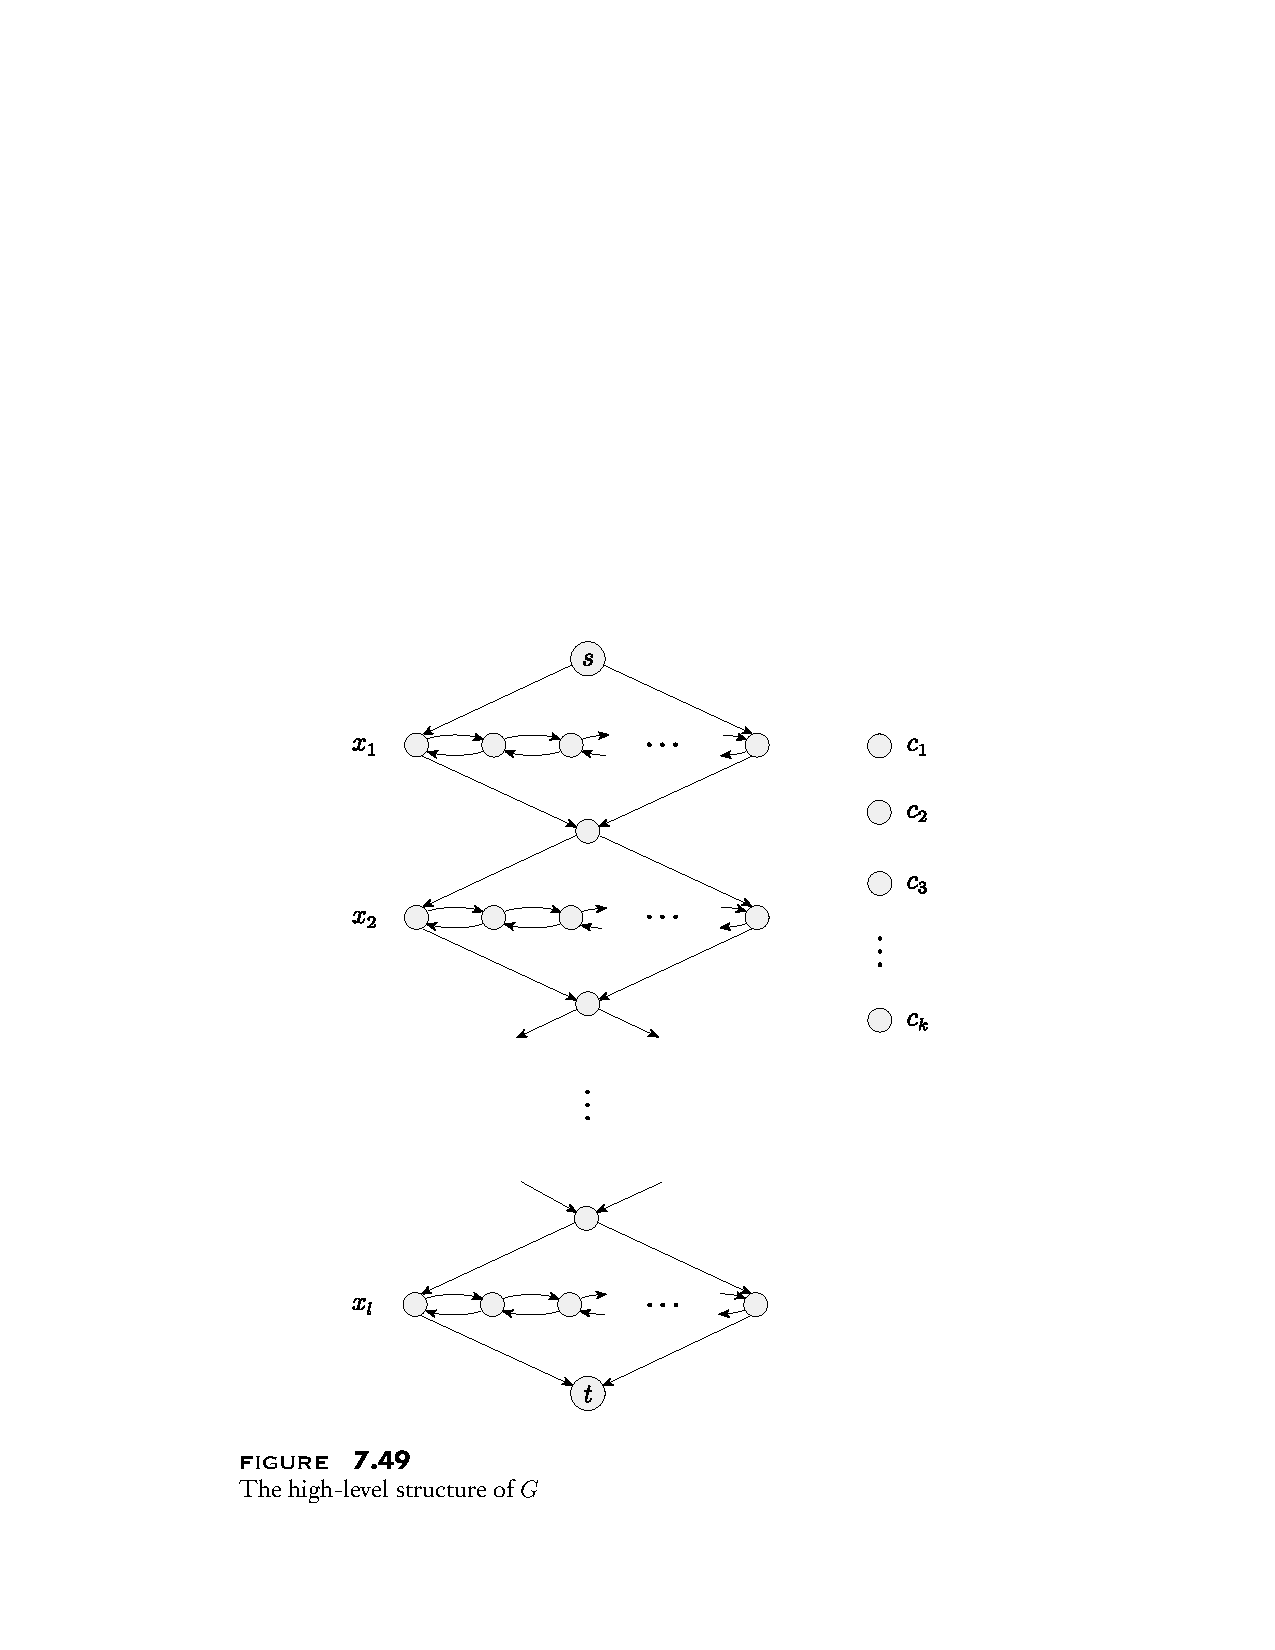
\includegraphics[width=0.5\textwidth]{ham-path-1}
    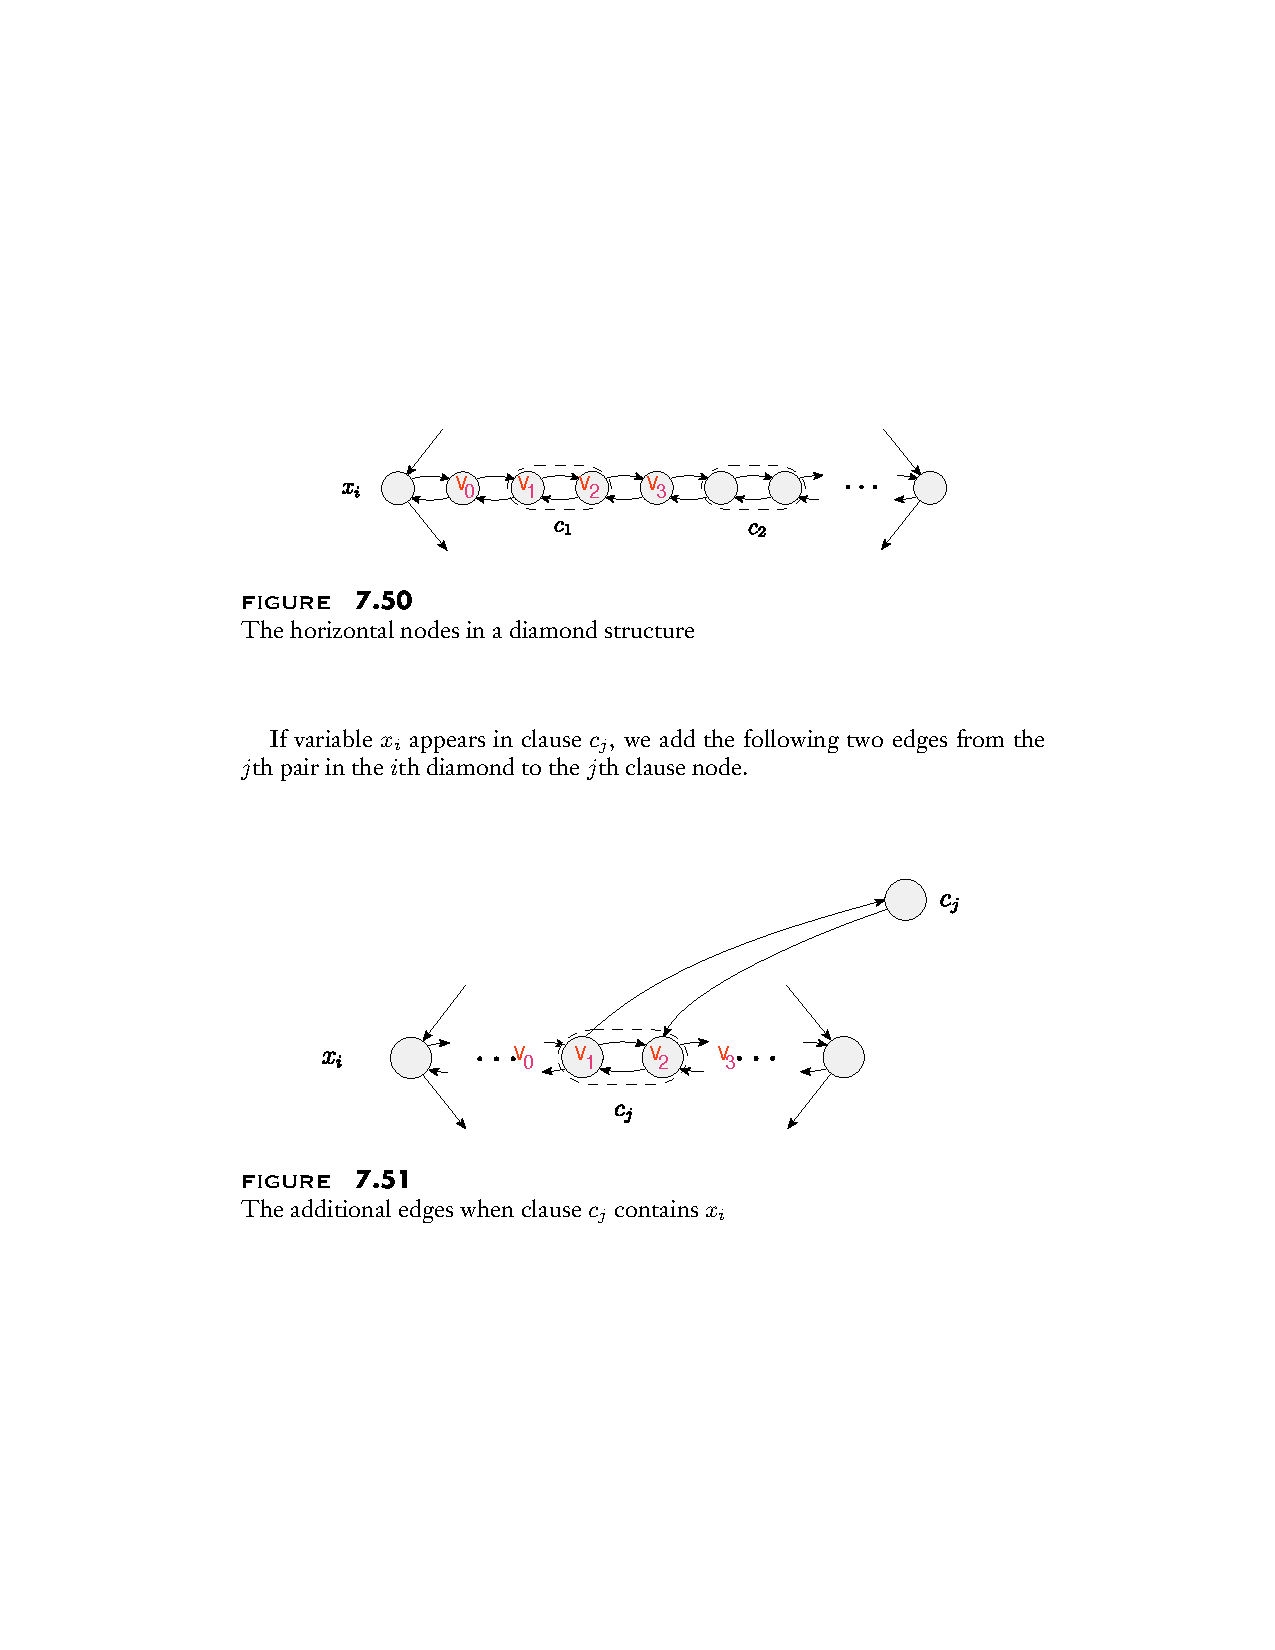
\includegraphics[width=0.55\textwidth]{ham-path-2}
    \caption{Figures 7.49--7.51 of Sipser's \emph{Introduction to the Theory of Computation}, \copyright\ Michael Sipser,
      reproduced here for commentary; they are not covered by these notes' license.}
  \end{figure}

  \paragraph{The reduction.}
  Given any instance $\phi$ of \prob{3-CNF-SAT},
  the reduction $f(\phi)$ outputs $(G, s, t)$
  where digraph $G$, source $s$, and sink $t$ are as
  shown in Figures~7.49--7.51.
  (We've borrowed these figures
  from the excellent text \emph{Theory of Computation}, by Sipser.)

  The global structure of $G$ is shown in Sipser's Fig.~7.49.
  Each variable $x_i$ in $\phi$ has a variable gadget in $G$.
  Each clause in $\phi$ has a clause gadget.
  The variable gadget for $x_i$ consists of 
  a long, doubly linked list of vertices
  with edges from each endpoint of the list to an intermediate vertex below.
  (See Sipser's Fig.~7.50.)
  % [review 2026-09-27] fix: the separator vertices, which the proof of the claim below relies on, were not described
  The vertices of the list come in groups: for each clause $c_j$ there is a pair of adjacent vertices,
  and between consecutive pairs, and at each end of the list, there is a \emph{separator} vertex,
  whose only edges are those of the list.
  The gadgets for the variables $x_1, x_2, \ldots, x_n$ are connected in sequence
  as shown in Fig.~7.49,
  ending with the sink $t$.

  For each clause $c_j$, the clause gadget has a single new vertex labeled $c_j$,
  and edges as shown in Fig.~7.51.
  For each literal $x$ or $\overline x$ in the clause,
  we select a unique adjacent pair of vertices $(u,w)$ in the variable gadget for $x$
  (where $u$ is to the left of $w$ in the list).
  If the literal is a variable $x$, we add edges from $u$ to the clause vertex $c_j$
  and from that vertex to $w$.
  Otherwise (the literal is a negation, $\overline x$),
  we add edges in the opposite direction: 
  from $w$ to the clause vertex and from the clause vertex to $u$.
  In either case,  we call the path from $u$ to $w$ (or vice versa) formed 
  by the two edges a \emph{detour}.

  This completes the reduction:
  given any \prob{3-CNF-SAT} formula $\phi$,
  the reduction produces the \prob{Hamiltonian Path} instance $f(\phi) = (G,s,t)$
  consisting of the graph $G$, source $s$ and sink $t$ described above.

  Clearly the reduction can be computed in time polynomial in $|\phi|$.

  \paragraph{Proof of correctness.}
  To finish, we need to prove that the reduction is correct.
  That is, we need to show
  \[(\forall \phi)~ \phi\in\prob{3-CNF-SAT} \iff f(\phi) \in \prob{Hamiltonian Path}.\]

  Consider any instance $\phi$ of \prob{3-CNF-SAT}.
  Let $(G, s, t) = f(\phi)$ as described above.
  
  \paragraph{Only if ($\implies$).}
  Suppose that $\phi$ is satisfiable.  
  We need to show that, in this case, $G$ has a Hamiltonian path $P$.
  Let $A$ be the assignment that satisfies $\phi$.
  Construct $P$ from $A$ as follows.

  Start at $s$.
  If $A$ assigns $x_1$ the value ``true'',
  then traverse the variable gadget for $x_1$ from left to right.
  Along the way, for each clause $c_j$ that contains the literal $x_1$,
  we will encounter a pair of adjacent vertices $u, w$ (in that order)
  such that $u$ has an edge to the clause vertex for $c_j$,
  which in turn has an edge back to $w$.  Take this ``detour''
  (the two edges) to visit the clause vertex, returning to $w$
  and continuing to traverse from left to right.

  Or, if $A$ assigns $x_1$ the value ``false'',
  then traverse the variable gadget for $x_1$ from \emph{right to left}.
  Along the way, for each clause $c_j$ that contains the literal $\overline{x_1}$,
  we will encounter a pair of adjacent vertices $u, w$ (in that order)
  such that $u$ has an edge to the clause vertex for $c_j$,
  which in turn has an edge back to $w$.  Take this ``detour''
  (the two edges) to visit the clause vertex, returning to $w$
  % [review 2026-09-27] fix: in the x_1 = false case the gadget is traversed right to left, so "continuing ... from left to right" was a copy-paste error; changed to right to left
  and continuing to traverse from right to left.
  
  Continue by, traversing the variable gadgets for $x_2$, $x_3$, etc.~similarly:
  (traverse the gadget for $x_i$ left-to-right if $A$ assigns $x_i$ the value ``true'',
  and otherwise right-to-left;
  detour to visit clause vertices that contain the corresponding 
  literal, unless the clause vertex has already been visited once).
  Stop when we reach $t$.
  In this way, we can traverse from $s$ to $t$, and visit each vertex exactly once.

  By this part of the proof,
  $\phi$ is satisfiable only if
  $G$ has a Hamiltonian path.

  \paragraph{If ($\impliedby$).}
  Suppose that $G$ has a Hamiltonian path $P$ from $s$ to $t$.
  We need to show that, in this case, $\phi$ has some satisfying assignment $A$.
  Construct $A$ from $P$ as follows.

  First, we argue that the path $P$ has to be \emph{well-formed}, meaning
  that it corresponds to some assignment.
  Specifically, $P$ must traverse the gadgets for variables $x_1,x_2,\ldots,x_n$, in order,
  and, for each $i$, must traverse the variable gadget for $x_i$ either left-to-right
  (with detours to clause gadgets of clauses that contain literal $x_i$)
  or right-to-left
  (with detours to clause gadgets of clauses that contain literal $\overline x_i$).

  We claim that
  \emph{if $P$ takes any edge on some detour, then it has to take the other edge as well.}

  Next we prove the claim.
  Note Figures 7.50 and 7.51.
  Consider any detour $(v_1,c_j,v_2)$ from the gadget for a variable $x_i$.
  Assume $v_1$ is just to the left of $v_2$ and clause $c_j$ contains literal $x_i$
  (the case when $v_1$ is just to the \emph{right} of $v_2$ 
  and clause $c_j$ contains literal $\overline{x_i}$ is similar).
  Let $v_0,v_1,v_2,v_3$ be the sub-path in the variable gadget around $v_1,v_2$.

  Vertex $v_3$ has only one neighbor other than $v_2$,
  so $P$ contains exactly one of the two edges $(v_2,v_3)$ or $(v_3,v_2)$.
  In the case that $P$ contains $(v_3,v_2)$, it also contains $(v_2,v_1)$
  (because no other edge leaves $v_2$).
  So (i) 
  \emph{$P$ contains either the edge $(v_2,v_3)$ or the sub-path $P_3 = (v_3,v_2,v_1)$.}

  Similarly, vertex $v_0$ has only one neighbor other than $v_1$,
  so $P$ contains exactly one of the two edges $(v_0,v_1)$ or $(v_1,v_0)$.
  In the case that $P$ contains $(v_1,v_0)$, it also contains $(v_2,v_1)$
  (because no other edge enters $v_1$).
  So (ii)
  \emph{$P$ contains either the edge $(v_0,v_1)$ or the sub-path $P_3' =(v_2,v_1,v_0)$.}

  First consider the case that \emph{$P$ contains $(v_2,v_3)$}.
  Then $P$ can't contain $P'_3$ (which has edge $(v_2,v_1)$),
  so by (ii) must contain $(v_0,v_1)$ along with $(v_2,v_3)$.
  If $P$ also happens to contain $(v_1,v_2)$, 
  then $P$ can't contain either edge of the detour.
  Otherwise ($P$ does not contain $(v_1,v_2)$),
  $P$ has to contain the first edge of the detour
  because that is the only way left out of $v_1$,
  and it has to contain the second edge of the detour
  (because that is the only way left into $v_2$).
  So, if $P$ contains $(v_2,v_3)$, then the claim holds.

  Next consider the remaining case, by (i):
  \emph{$P$ contains $P_3=(v_3,v_2,v_1)$}.
  Then $P$ can't contain $(v_0,v_1)$ (because $P$ contains $(v_2,v_1)$),
  so by (ii) must contain $P'_3=(v_2,v_1,v_0)$ as well as $P_3$,
  so must contain sub-path $(v_3,v_2,v_1,v_0)$,
  and cannot contain either edge of the detour.
  So the claim holds in this case as well.
  This completes the proof of the claim.
  
  We now finish the proof that $\phi$ has a satisfying assignment $A$.
  Since, for each detour, $P$ contains either both edges of the detour or neither,
  replacing each detour $(v_1,c_j,v_2)$ from $P$ by the edge $(v_1,v_2)$
  gives a path $P'$ that visits all the nodes except the clause nodes.
  Considering the global structure of $G$ (Fig.~7.49), this path $P'$ 
  must traverse the gadgets for the variables $x_1, x_2, \ldots, x_n$
  in sequence, and must traverse each gadget either left-to-right
  or right-to-left.  Let $A$ assign the value ``true'' to each variable
  $x_i$ whose gadget $P'$ traverses left-to-right.
  Let $A$ assign ``false'' to each variable $x_i$
  whose gadget $P'$ traverses right-to-left.
  This is assignment assigns values to all the variables.
  To see that the assignment has to satisfy $\phi$,
  consider any clause $c_j$.
  The original path $P$ traversed this clause,
  and (by the claim) did so via some detour 
  $(v_1,c_j,v_2)$ from the gadget of a variable $x_i$
  such that $x_i$ or $\overline x_i$ occurs in clause $c_j$.
  Consider the case that $x_i$ occurs in clause $c_j$.
  (The case when $\overline x_i$ occurs in the clause is similar.)
  Then, by the construction of $G$, 
  in the detour $v_1$ is just to the left of $v_2$,
  which (considering $P'$ and the claim)
  means that $P'$ must traverse the gadget for $x_i$
  left-to-right, which by the way $A$ is constructed
  that $A$ assigns variable $x_i$ value ``true'',
  so $A$ satisfies clause $c_j$.

  By this part of the proof,
  if $G$ has a Hamiltonian path
  then $\phi$ is satisfiable.

  \smallskip

  By the parts of the proof above,
  for all 3-CNF formulas $\phi$,
  $\phi$ is satisfiable
  if and only if
  $f(\phi)$ has a Hamiltonian path.
  Therefore, the reduction is correct.
\end{proof}

\section{External sources on P, NP, and NP-completeness}\label{np: sec: external}\doHeader{External sources}


\begin{itemize}
\item \DPV~Chapter 8.  \JE Chapter 12. \KT Chapter 8 (and \KWSlides). \CLRS Chapter 34.  MIT video:
  

\URL{https://ocw.mit.edu/courses/electrical-engineering-and-computer-science/6-006-introduction-to-algorithms-fall-2011/lecture-videos/lecture-23-computational-complexity/}

\item Chapter 7.3 of \href{https://www.google.com/search?client=safari&rls=en&q=sipser+theory+of+computation+3rd+edition+pdf&ie=UTF-8&oe=UTF-8}{Sipser's \emph{Theory of Computation}}

\end{itemize}

\end{document}

%%% Local Variables:
%%% mode: latex
%%% TeX-master: t
%%% End:
